\section{Extensive games}

\begin{definition}[\textit{Extensive form game with perfect information}]
    An extensive form game with perfect information consists of:
\end{definition}
\begin{enumerate}
    \item A finite set $N = \{1,\dots,n\}$ of players. 
    \item A game tree $(V,E,x_0)$.
    \item A partition of the non-leaf vertices into sets ${P1, P2, \dots , Pn+1}$.
    \item A probability distribution for each vertex in $P_{n+1}$, defined on the edges from that vertex to its children.
\end{enumerate}
The game includes the following:
\begin{enumerate}
    \item The set $P_i$, for $i \leq n$, consists of nodes where Player $i$ must choose a child of $v$, representing a possible move by that player.
    \item $P_{n+1}$ is the set of nodes where chance plays a role (i.e., random events). 
        Here, $n + 1$ refers to the players plus the random component. $P_{n+1}$ can be empty, indicating no random events in the game.
    \item When $P_{n+1}$ is empty, the $n$ players only have preferences over the leaves, meaning no random component influences the outcome, so a utility function isn't required.
\end{enumerate}

\subsection{Extensive game solution}
To determine the optimal outcome, we apply the axioms of rationality.
\begin{example}
    For the voting game described earlier:
    \begin{figure}[H]
        \centering
        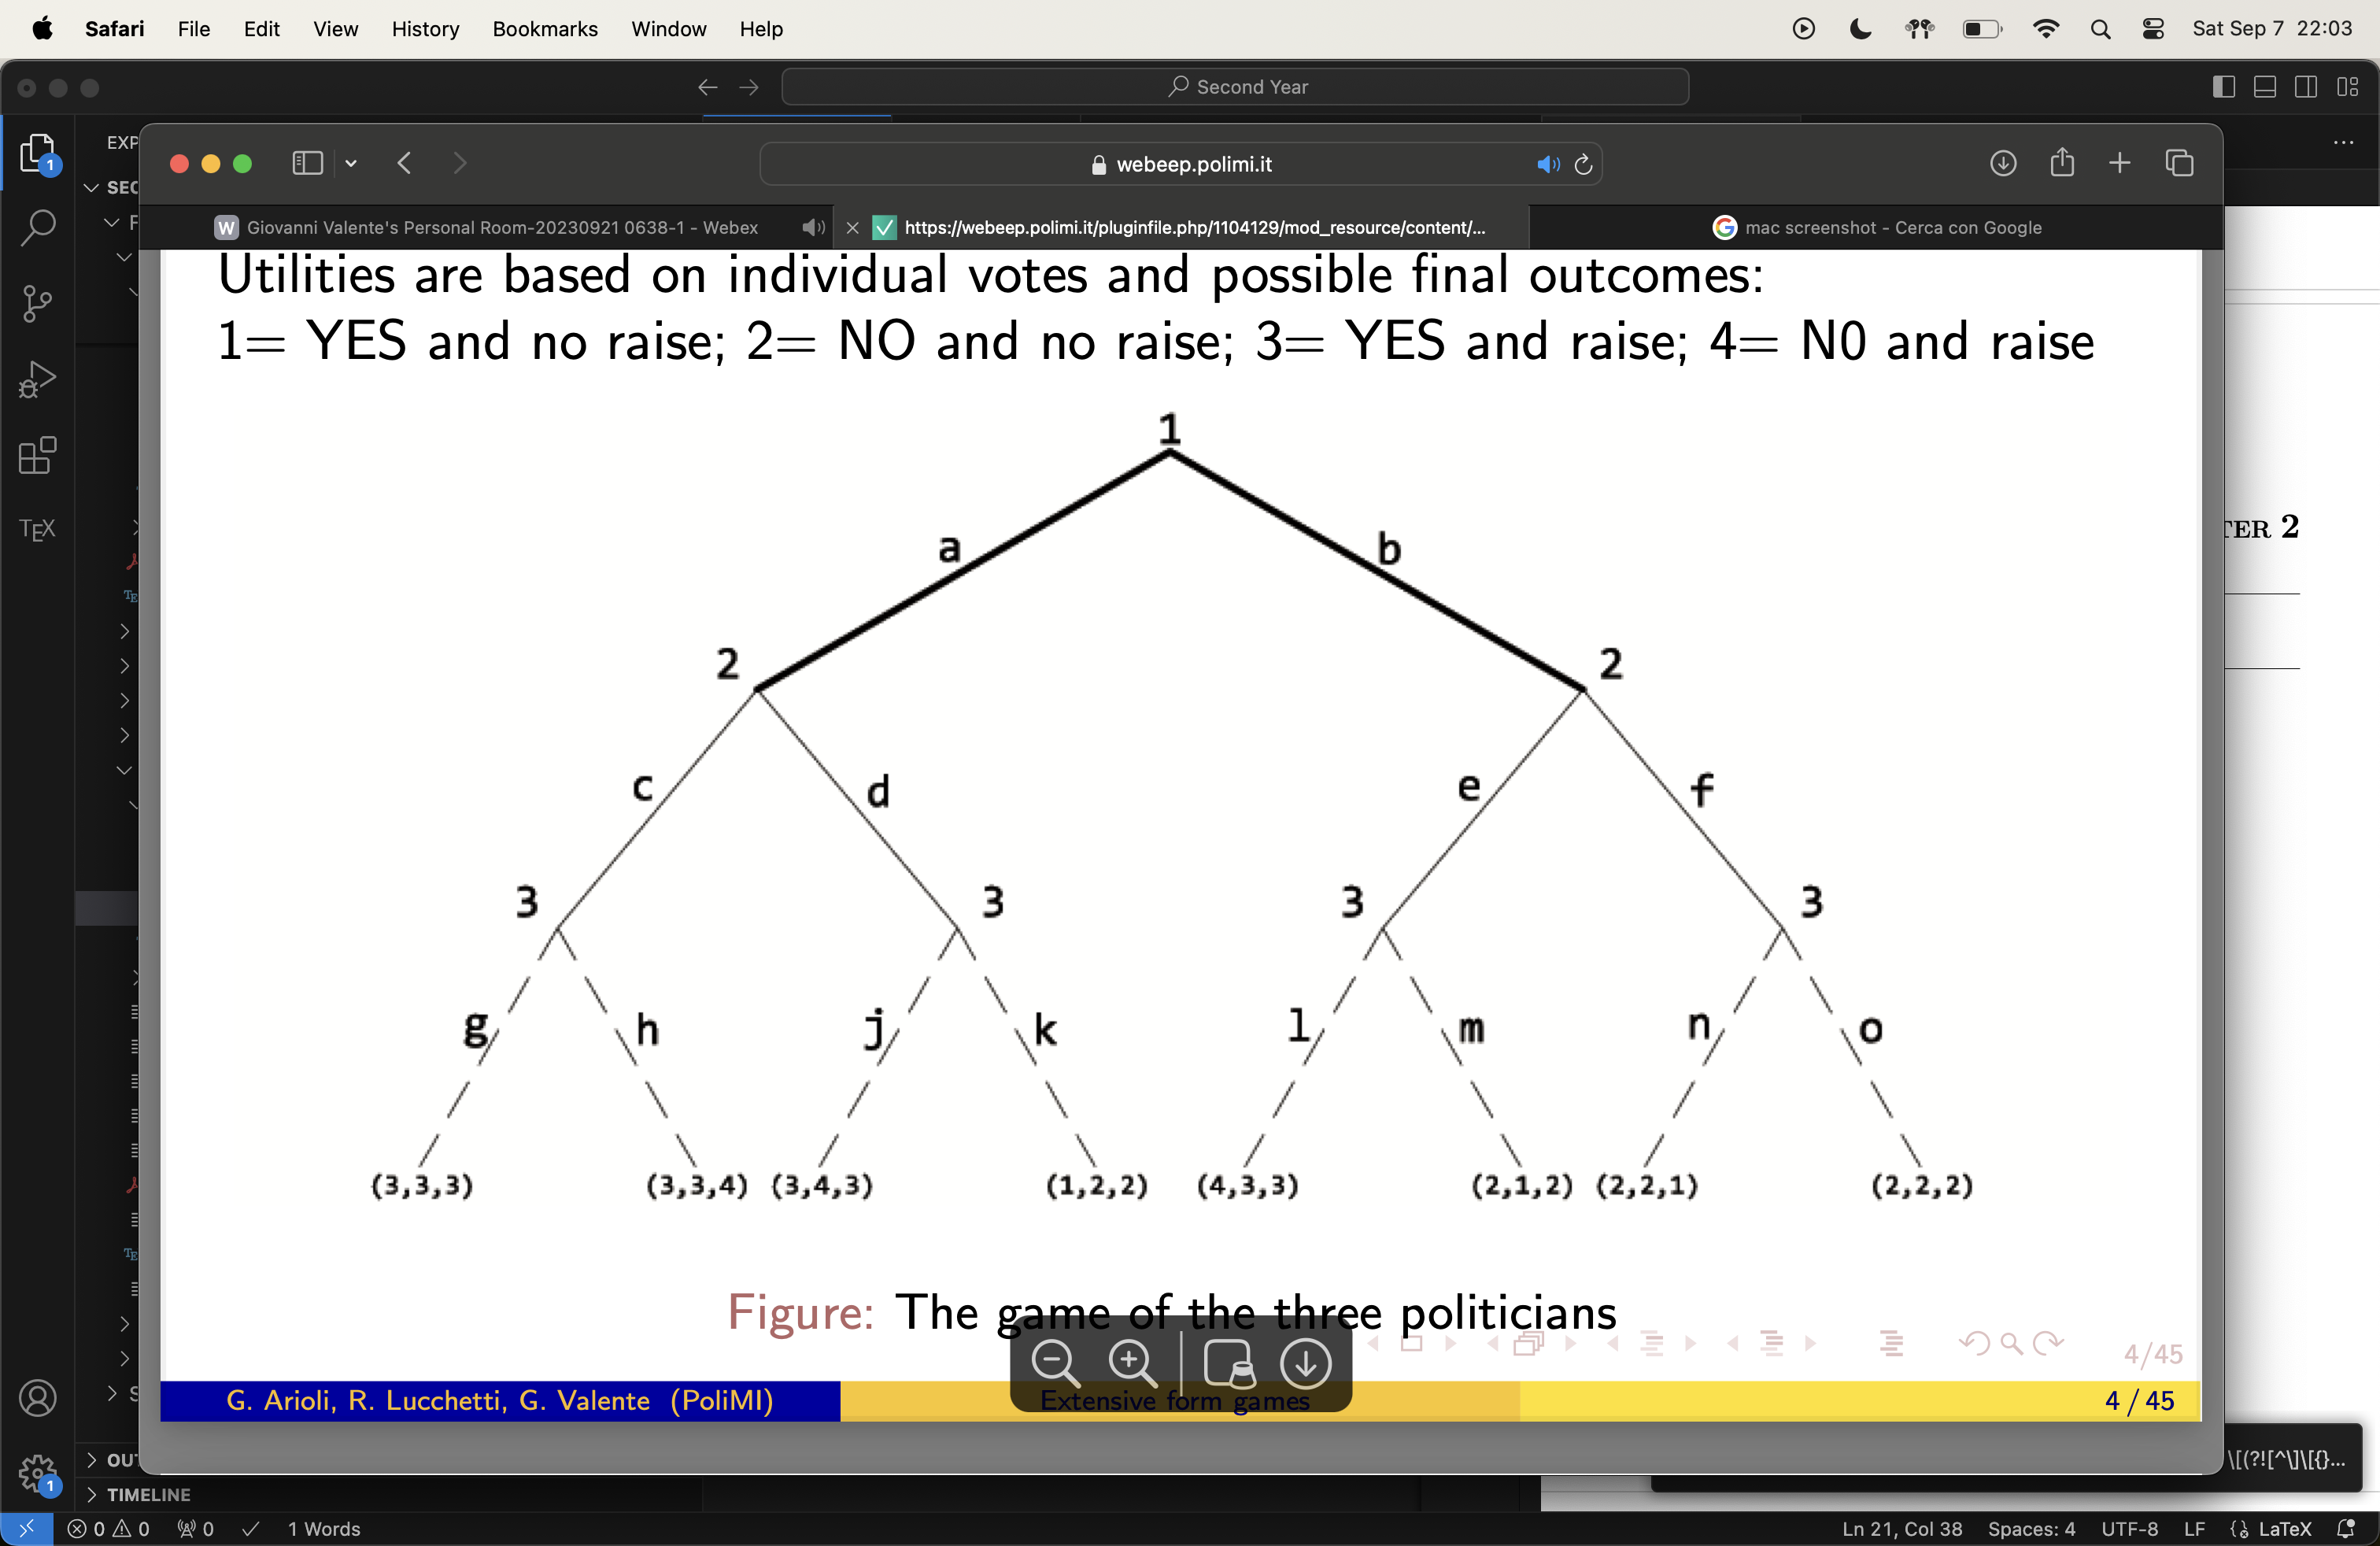
\includegraphics[width=0.75\linewidth]{images/tree.png}
        \caption{Voting game tree}
    \end{figure}
    We can identify the preferences as follows:
    \begin{itemize}
        \item For Player 3: 
            \begin{itemize}
                \item $h = \begin{pmatrix} 3 & 3 & 4 \end{pmatrix}$ over $g = \begin{pmatrix} 3 & 3 & 3 \end{pmatrix}$.
                \item $j = \begin{pmatrix} 3 & 4 & 3 \end{pmatrix}$ over $k = \begin{pmatrix} 1 & 2 & 2 \end{pmatrix}$.
                \item $l = \begin{pmatrix} 4 & 3 & 3 \end{pmatrix}$ over $m = \begin{pmatrix} 2 & 1 & 2 \end{pmatrix}$.
                \item $o = \begin{pmatrix} 2 & 2 & 2 \end{pmatrix}$ over $n = \begin{pmatrix} 2 & 2 & 1 \end{pmatrix}$.
            \end{itemize}
        \item For Player 2: 
            \begin{itemize}
                \item $d = \begin{pmatrix} 3 & 4 & 3 \end{pmatrix}$ over $c = \begin{pmatrix} 3 & 3 & 4 \end{pmatrix}$.
                \item $e = \begin{pmatrix} 4 & 3 & 3 \end{pmatrix}$ over $f = \begin{pmatrix} 2 & 2 & 2 \end{pmatrix}$.
            \end{itemize}
        \item For Player 1:
            \begin{itemize}
                \item $b = \begin{pmatrix} 4 & 3 & 3 \end{pmatrix}$ over $a = \begin{pmatrix} 3 & 4 & 3 \end{pmatrix}$.
            \end{itemize}
    \end{itemize}
    Thus, the optimal outcome is found. 
\end{example}
\begin{definition}[\textit{Length}]
    The length of a game is defined as the length of the longest path in the game tree.
\end{definition}
Using decision theory and the assumption of rationality:
\begin{itemize}
    \item Rationality assumption 5 allows us to solve games of length 1.
    \item Rationality assumption 4 allows us to solve games of length $i + 1$ if all games of length at most $i$ have already been solved.
\end{itemize}
This iterative process is called backward induction, where we work backwards from the leaves of the tree to the root to determine the optimal sequence of actions.
\begin{theorem}[First rationality theorem]
    The rational outcomes of a finite game with perfect information are those determined by the backward induction procedure.
\end{theorem}
Backward induction can be applied because every vertex $v$ in the game is the root of a subgame consisting of all the vertices that follow $v$. 
These subgames are derived from the original game.
\begin{example}
    For the chance game: 
    \begin{figure}[H]
        \centering
        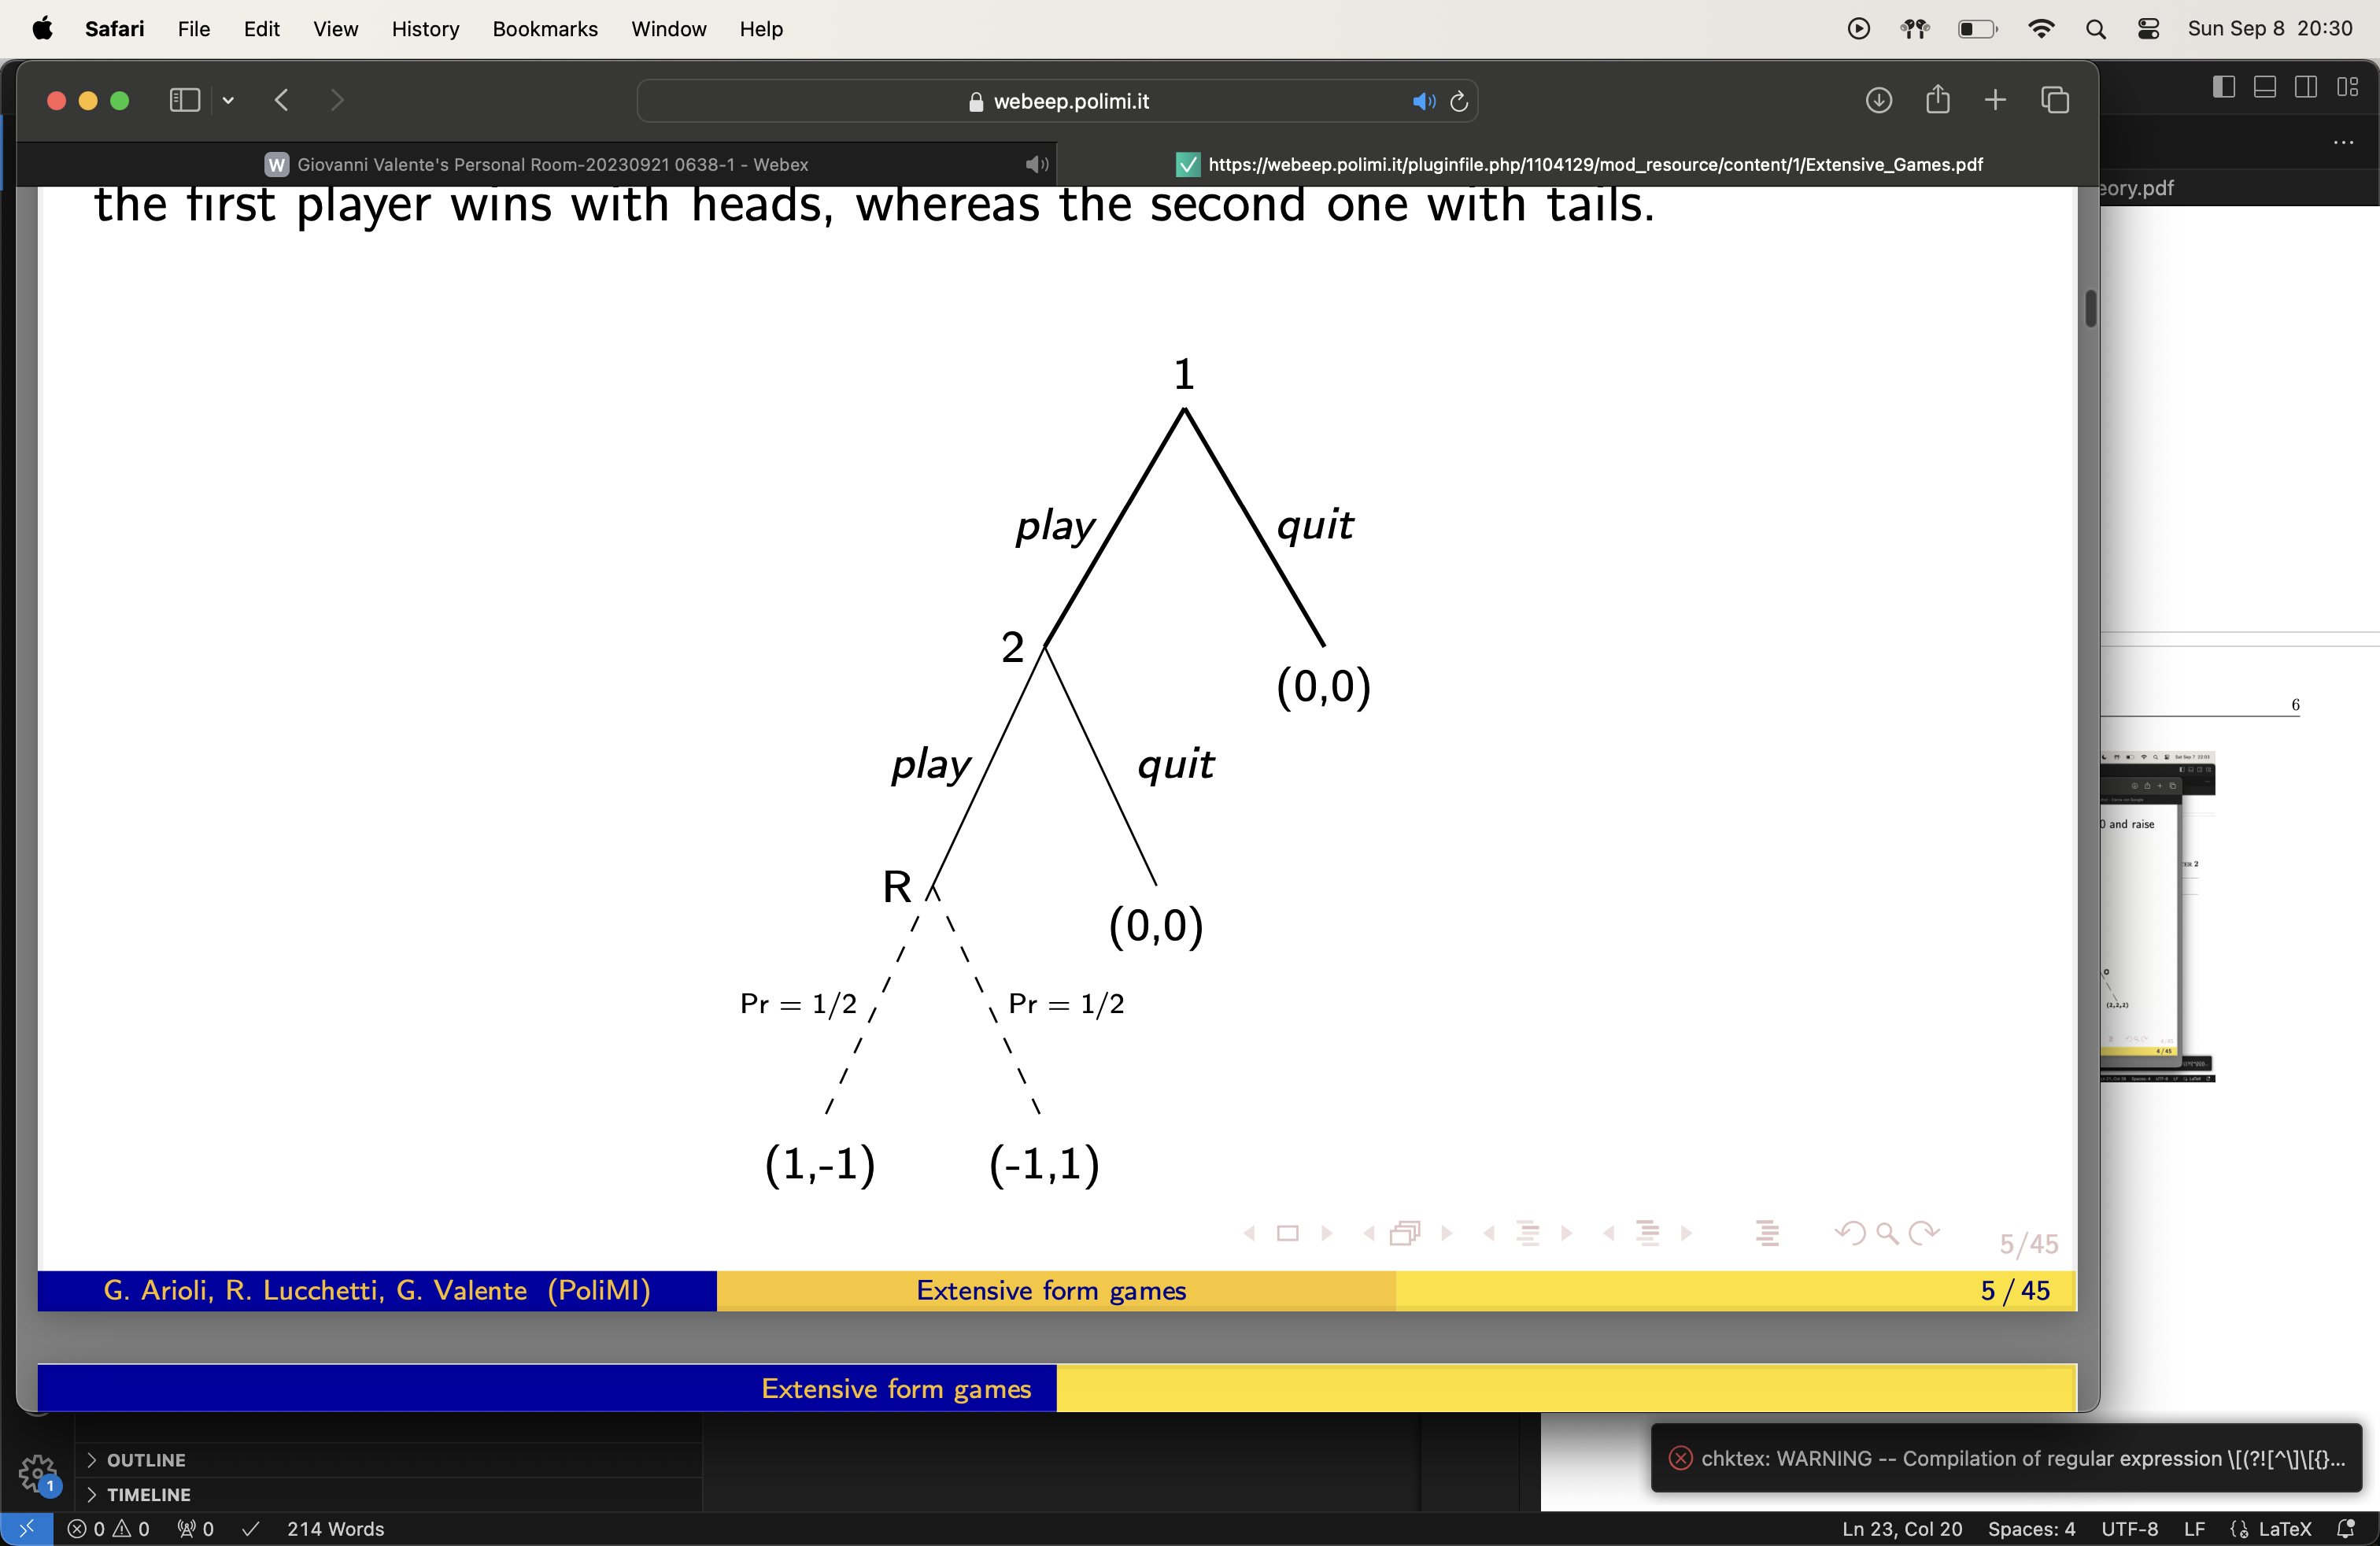
\includegraphics[width=0.75\linewidth]{images/tree1.png}
        \caption{Chance game tree}
    \end{figure}
    The outcomes obtained through backward induction are $\begin{pmatrix} 4 & 3 \end{pmatrix}$ and $\begin{pmatrix} 3 & 4 \end{pmatrix}$. 
    Player 2 has no strict preference between $\begin{pmatrix} 4 & 3 \end{pmatrix}$ and $\begin{pmatrix} 0 & 3 \end{pmatrix}$, indicating that in general, the solutions may not be unique.
\end{example}